\documentclass[]{elsarticle}

\usepackage[T1]{fontenc}
\usepackage{multicol}
\usepackage{graphicx}
\usepackage[margin=0.8in]{geometry}
\usepackage{color}
\PassOptionsToPackage{hyphens}{url}\usepackage{hyperref}
\usepackage[usenames,dvipsnames,svgnames,table]{xcolor}
\hypersetup{colorlinks=true, citecolor=blue}

\usepackage{tocloft}
\usepackage{float}

\makeatletter
\def\ps@pprintTitle{%
	\let\@oddhead\@empty
	\let\@evenhead\@empty
	\let\@oddfoot\@empty
	\let\@evenfoot\@oddfoot
}
\makeatother

%opening

\begin{document}
	
	\onecolumn
	
	\begin{abstract}
		\par The use of multi-spectral images is growing rapidly in the field of precision agriculture,
		and is currently based on the use of multi-sensor cameras such as the airphen camera (6 spectral bands) or the sequoia (4 spectral bands).
		However, their use was still limited to high altitudes per drone ($\approx 150$ meters).
		As part of the reduction of phytosanitary measures,
		this type of device becomes necessary in order to discriminate crops and weeds in close detection ($< 10$ meters)
		in order to treat them as closely as possible in order to directly target the plants.
		Which requires high spatial resolution to calculate spectral index and extract information such as shape, texture, \dots for weed classification.
		\\
		\par The problem with these cameras is that not all sensors are aligned and the manufacturers' methods are not adapted.
		We therefore need a solution to align the different images accurately in close-view.
		The objective of this article is to propose a simple method for agronomic scenes that allows to define the ideal conditions
		for matching multi-spectral images from the multi-sensor camera at low heights of use.
		\\
		\par In this study we propose a two steps method applied to the aiphen multi-sensors camera :
		(i) Affine correction using pre-calibrated matrix at different height, the closest transformation can be selected via internal GPS.
		And (ii) Perspective correction to refine the previous one, using keypoints matching between enhanced gradients of each spectral bands.
		Different types of keypoints detection, their benchmark and the best reference spectra are evaluated.
	\end{abstract}
	
	\begin{keyword}
		Registration \sep
		Multi-spectral imagery \sep
		Precision farming \sep
		Feature descriptor
	\end{keyword}
	
	\begin{frontmatter}
		\title{Two steep multi-spectral registration \\ via keypoint detector and gradient similarity}
		\author[unilu]{Jehan-Antoine VAYSSADE} \ead{jehan-antoine.vayssade@inra.fr}
		\author[unilu]{Christelle Gee} \ead{christelle.gee@agrosupdijon.fr}
		\address[myuni]{Agroécologie, AgroSup Dijon, INRA, Univ. Bourgogne, Univ. Bourgogne Franche-Comté,  F-21000 Dijon, France}
		\date{Received: date / Accepted: date}
	\end{frontmatter}
	
	\newpage
	
	\section{Introduction}
	
	\par Modern agriculture is changing towards a system that is less dependent on pesticides \cite{10.1371/journal.pone.0097922} (herbicides remain the most difficult pesticides to reduce) and increasingly uses digital tools. The development of imaging and image processing has made it possible to characterize an agricultural plot (the health status of a stand or characterize a soil) using non-destructive agronomic indices (NDVI, ExcessGreen, SBI, etc.) replacing traditional destructive and time-consuming methods. In recent years, the arrival of miniaturized multi-spectral and hyper-spectral cameras on mobile aerial platforms (UAVs) has made it possible to monitor a plot spatio-temporally. These vision systems have been developed for precise working conditions (flight height 150m). Although, very practical to use, they are also used for proxy-sensing applications. However, the algorithms for correcting and matching multiple single-band images of different spectral range, proposed by some manufacturers, are not optimal for low heights. To do so, an image registration is necessary.
	\\
	\par Image registration is the process of transforming different images of one scene into the same coordinate system.
	The spatial relationships between these images can be rigid (translations and rotations), affine (shears for example),
	homography, or complex large deformation models (due to the difference of depth between ground and leafs) \cite{Kamoun}.
	The main difficulty is that multi-spectral images have wavelength with high distance between each spectral bands.
	Which implies (i) leaves have a different aspect depending on the spectral bands
	(ii) there are highly complex and self-similar structures in our images
	(iii) and the scene are a grassland or agriculture image at different scale,
	which is a complex spectral scene making a hard fit for such a registration.
	\\
	\par There is two types of registration, feature based and intensity based \cite{Zitova}.
	(i) Feature based methods use feature matching, in most cases a bruteforce matching is used, making those techniques slow.
	Fortunately these features can be filtered to reduce the matching cost depending of the spatial properties we have, and a GPGPU implementation can reduce the comparisons cost.
	(ii) Intensity-based automatic image registration is an iterative process, and the metrics used are sensitive to determine the numbers of iteration,
	making such method even worth in time for precise registration. Furthermore in multi-spectral we need different metrics for each registered bands which is hard to achieve.
	\\
	\par Different studies of images alignment using multi-sensors camera exist using UAV at high distance.
	Some show good performances for feature based \cite{DantasDiasJunior, Vakalopoulou} with strong enhancement of feature descriptor for matching performances.
	Other don't and prefer to use intensity based \cite{douarre:hal-02183837} with better convergence metrics, which is slower and not necessarily robust against light variability.
	\\
	\par Unless this type of articles, the domain is not very well sourced, no studies have been made under agricultural and external conditions in near field of view (less than 10 meter).
	Those studies mainly propose features matching without large methods comparison of their performance (time/precision),
	spectral band reference selection, or pre-affine correction depending on the distance.
	Thus, this study propose the best combination of feature extractor and spectral reference on normalized gradients transformation,
	using pre-affine registration and matches filtering, evaluated at different spatial resolution.
	%\\
	%\par In this study we have preferred not to enhance features by the information send to each features methods,
	%as example SIFT have been rejected on the paper \cite{douarre:hal-02183837}
	%which explain that the matched features are two numerous and not greatly matched.
	
	\section{Material and Method}
	
	\subsection{Material}
	
	The multi-spectral imagery was provided by the six-band multi-spectral camera Airphen \footnote{\url{https://www.hiphen-plant.com/our-solutions/airphen/}}.
	AIRPHEN is a scientific multi spectral camera developed by agronomists for agricultural applications.
	It can be embedded in different types of platforms such as UAV, phenotyping robots, etc.
	\\
	\par AIRPHEN is highly configurable (bands, fields of view), lightweight and compact.
	It can be operated wireless and combined with complementary thermal infrared channel and high resolution RGB cameras.
	The camera was configured using 450/570/675/710/730/850 nm with FWHM of 10nm.
	The focal lens is 8mm. It's raw resolution for each spectral band is 1280x960 px with 12 bit of precision.
	Finally the camera also provide an internal GPS antenna, that can be used to get the distance from the ground.
	\\
	\par Two datasets were taken at different heights.
	We have used a metallic gantry for positioning the camera at different heights.
	The size of the gantry is about $3m * 5m * 4m$.
	Due to the size of the chessboard, the limited focus of the camera and the height of the gantry,
	we have bounded the acquisition height from 1.6 meter to 5 meter with 20cm steep, which represent 18 acquisitions.
	\\
	\par The first dataset is for the calibration. A chessboard is taken at different heights, the corresponding data can be found in data/steep-chess/.
	The second one is for the alignment verification under reel condition.
	One shot of an agronomic scene is taken at different heights, the corresponding data can be found in data/steep/
	with a bias of +/- 10cm to be in the worst case (most complex).
	
	\subsection{Methods}
	
	Alignment is refined in two stages, with
	(i) affine registration roughly estimated
	and (ii) perspective registration for the refinement and precision.
	%As example the figure \ref{fig:merged-correction} show each correction steep at 1.6 meters.
	%
	%\begin{figure}[!htb]
	%	\centering
	%	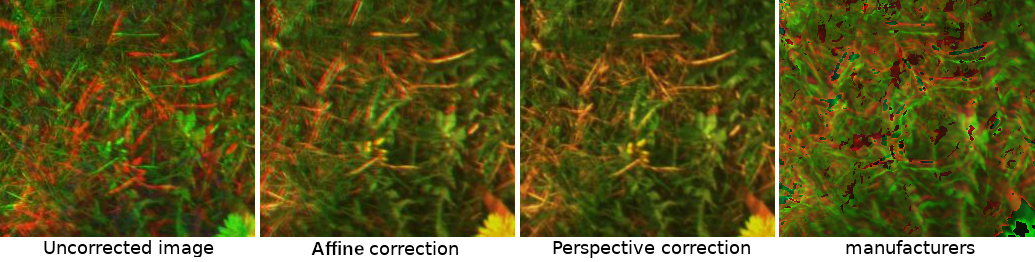
\includegraphics[width=\linewidth]{../figures/merged-correction.png}
	%	\caption{Exemple of each correction}
	%	\label{fig:merged-correction}
	%\end{figure}
	
	\subsubsection{Affine Correction}
	
	It's important to notice the closer we take the snapshot, the bigger is the distance of the initial Affine Correction.
	On the other hand at a distance superior or equals to 5 meters, the initial affine correction become stable (figure \ref{fig:affine-translation-height}).
	A calibration is used to build a linear model, which makes the affine correction to work at any height.
	The main purpose of this step is to reduce the distance of each spectral band,
	which allow the similarity to be spatially delimited within a few pixels, making feature matching more effective.
	
	\paragraph{Calibration}
	We use opencv 4 \textit{findChessboardCorners} for each spectral image (normalized) at different heights (from 1.6 to 5 meters).
	The function attempts to determine whether the input image is a view of the chessboard pattern and locate the internal chessboard corners.
	The detected coordinates are approximated, and to determine their positions more accurately we use the function \textit{cornerSubPix} as explained in the documentation.
	The detected points are ordered by x/y (detection can be flipped) and saved on data/'height'.npy
	
	\paragraph{Making linear model}
	
	Using all the points detected for each spectral band, we calculate the centroid grid (each point average).
	The affine transform from each spectral band to this centroid grid is estimated.
	It appear that the rotation and the scale do not depend on the distance to the ground, but only on the translation.
	%This is expected, so that only one calibration can be used for this part of the matrix.
	%The rotation and scale factor that is quite stable and close to identity (accuracy depends on the spatial resolution of the board).
	On the other hand, the translation in $x, y$ depend on the height.
	Thus a Levenberg-Marquardt curve fitting algorithm with linear least squares regression \cite{More78}
	can be used to fit an equation for each spectral band again $x$ and $y$ independently to the centroid grid.
	We have chosen to adjust the following curve $y = ax^3 + bx^2 + cx + d$ where $x$ is the height,
	$y$ is the resulted translation and factors $a,b,c,d$ are the model parameter.
	%The fitted parameters for each spectral bands can be found in supplementary data.
	
	\paragraph{Correction}
	
	To make the affine matrix correction, we used the rotation and scale factors at the most accurate height (1.6 meter), because it doesn't depend on the height.
	For the translation part, the curve model is applied for each spectral bands at the given height (roughly known by the user or using the internal GPS sensor).
	Each spectral band are so warped using the corresponding affine transformation.
	Finally, all spectral bands are cropped to the minimal bounding box (minimal and maximal translation of each affine matrix).
	
	\subsubsection{Perspective correction}
	%Once the best keypoints extractor and spectral reference are defined, we use there detection to estimate an homography.
	%Homography is an isomorphism of perspectives. A 2D homography between A and B would give you the projection transformation
	%between the two images. It is a 3x3 matrix that describes the affine transformation.
	
	
	Each spectral band has different properties and values by nature. (figure \ref{fig:vegetable-gradient})
	But we can extract the corresponding similarity by transforming each spectral band into its absolute derivative,
	to find similarity in gradient break among them.
	
	\begin{figure}[H]
		\centering
		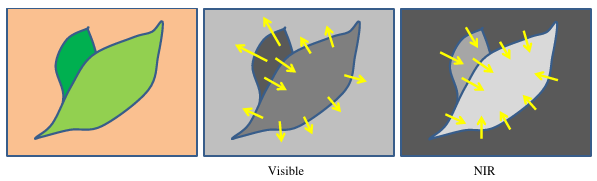
\includegraphics[width=0.6\linewidth]{../figures/contrast-inversion.png}
		\caption{
			Gradient orientation in spectral band \cite{rabatel:hal-01684135},
			we can see that the orientation of the gradient is not the same depending to the spectral band,
			making the absolute derivative an important step for matching between different spectral band.
		}
		\label{fig:vegetable-gradient}
	\end{figure}
	
	\par The previous correction, such as Affine correction attempts to help the feature matching by adding properties of epipolar lines (close).
	Thus, the correspondence of the extracted features can be spatially bounded,
	(i) we know that the maximum translation is limited to a distance of a few pixels (less than $10$px),
	and (ii) the angle between the initial element and the matched one is limited to $[-1,1]$ degree.
	
	\paragraph{Computing the gradient} To compute the gradient of the image with a minimal impact of the light distribution (shadow, reflectance, specular, ...)
	Each spectral band are normalized using Gaussian blur \cite{sage0303}, the kernel size is defined by $math.ceil(image\_width^{0.4}) // 2 * 2 +1$ (19 in your case)
	and the final normalized image are defined by $i/(G+1)*255$ where $i$ is the spectral band and $G$ is the Gaussian blur of those spectral band.
	This first steep allow to minimize the impact of the noise on the gradient and smoothes the signal in case of hight reflectance.
	Using this normalized image, the gradient is computed with the sum of Sharr filter \cite{Seitz} again $d_x=1$ and $d_y=1$.
	%Different types of edge detection such as Sobel, Laplacan and Canny were tested unsuccessfully (without sufficient number of matches), those not included in this study.
	Finally, all gradients are normalized using CLAHE \cite{zuiderveld1994contrast} to locally improve their intensity and increase the number of key points detected (especially for 850nm).
	%\begin{figure}[!htb]
	%	\centering
	%	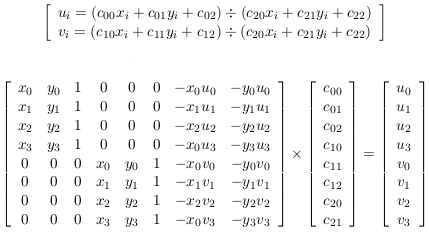
\includegraphics[width=0.6\linewidth]{../figures/math-perspective-correction.png}
	%	\caption{equation of the perspective correction}
	%	\label{eq:perspective}
	%\end{figure}
	
	\paragraph{Keypoints Extractor}
	A key point is a point of interest. It defines what is important and distinctive in an image.
	Different types of key point extractors were tested, all the results can be found in "figures/*".
	
	\begin{itemize}
		\item ORB : An efficient alternative to SIFT or SURF
		\item AKAZE : Fast explicit diffusion for accelerated features in nonlinear scale spaces
		\item KAZE : A novel multi-scale 2D feature detection and description algorithm in nonlinear scale spaces \cite{rs10050756}
		\item BRISK : Binary robust invariant scalable keypoints.
		\item AGAST : Adaptive and generic corner detection based on the accelerated segment test
		\item MSER : maximally stable extremal regions
		\item SURF : Speed-Up Robust Features
		\item FAST : FAST Algorithm for Corner Detection
		\item GFTT : Good Features to Track
	\end{itemize}

	These algorithms are all available and easily usable in OpenCV, the table \ref{tab:used-algorithms} in appendix
	show all tested algorithms. These algorithms were studied by varying the most influential parameters for each of them.
	
	\paragraph{Keypoint detection}
	We use one of the keypoint extractors mentioned above between each spectral band gradient (all extractors are evaluated).
	For each detected keypoint, we extract a descriptor using ORB features.
	We match all detected keypoints to a reference spectral band (all bands are evaluated).
	All matches are filtered (distance, position, angle) to eliminate false positives along the epipolar line.
	Finally we use the function \textit{findHomography} between the key points detected/filtered with RANSAC,
	to determine the best subset of matches to calculate the perspective correction.
	
	%\begin{figure}[!htb]
	%	\centering
	%	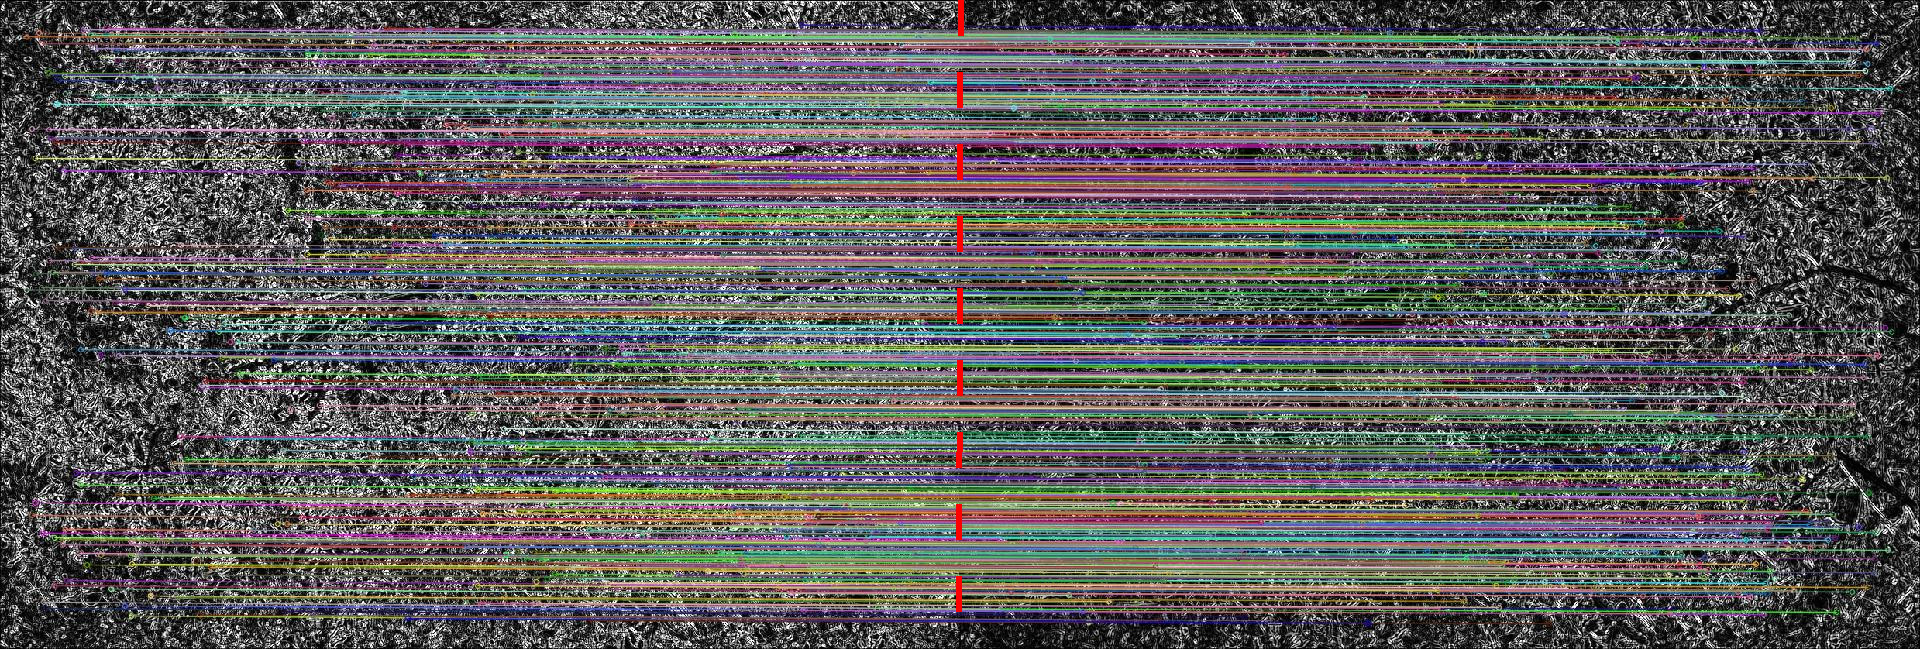
\includegraphics[width=0.7\linewidth]{../figures/prespective-feature-matching.jpg}
	%	\caption{feature matching}
	%	\label{fig:feature-matching}
	%\end{figure}
	
	\paragraph{Correction}
	
	The perspective correction between each spectral band to the reference is estimated and applied.
	Finally, all spectral bands are cropped to the minimum bbox,
	the minimum and maximum points are obtained by applying a perspective transformation to each corner of the image.
	
	%\subsection{Re-estimating the reel height}
	%The same procedure about curve fitting \cite{More78} can be used to evaluate the inverse model between height and translation.
	%By adding the affine translation and the perspective transform of the central image point $x,y$,
	%the ``real'' translation can be evaluate. Using this value as input of the inverse model,
	%we can estimate the real height of the acquisition.
	%
	%\noindent
	%\colorbox{green}{estimating the height of each spectral bands corner} \\
	%\colorbox{green}{to the reference can enable to build the ground plan ?} \\
	%\colorbox{green}{and enable to correct the row gradient ?}
	
	\section{Result and discussion}
	
	Firstly the results will focus on affine corrections and then on the effects of the perspective correction.
	As example the figure \ref{fig:merged-correction} show each correction steep at 1.6 meters and the manufacturer results.
	
	\begin{figure}[H]
		\centering
		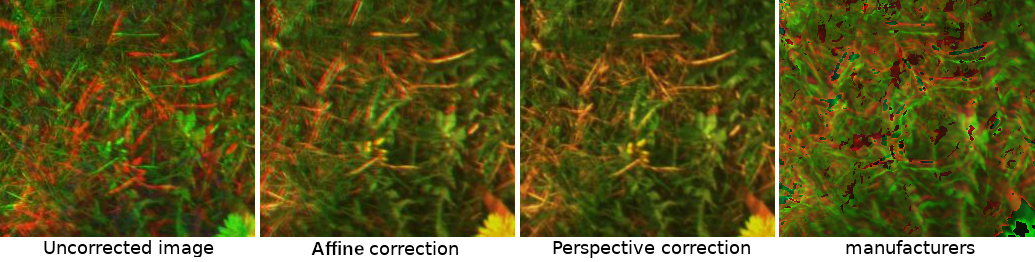
\includegraphics[width=0.7\linewidth]{../figures/merged-correction.png}
		\caption{Exemple of each correction and manufacturer}
		\label{fig:merged-correction}
	\end{figure}
	
	\subsection{Affine correction}
	
	The 6 coefficients ($A,B,C,D,X,Y$) of the affine matrix were studied according to the height of the camera in order to see their stability.
	It appears that the translation part ($X,Y$), depends to the distance of the field (appendix figure \ref{fig:affine-translation-height}).
	On this part the linear model are used to estimated the affine correction from an approximated height.
	%Due to the hard correlation between spectral bands these registration, especially between 450nm and 710-850nm (unless using normalized gradient)
	%have not been investigated and suggest that the reader should see the specific article \cite{rabatel:hal-01684135}.

	In other hand, rotation and scale do not depend on the ground distance (appendix figure \ref{fig:affine-rotation-height}).
	These factors ($A,B,C,D$) is quite stable and close to identity (accuracy depends on the spatial resolution of the board).
	Which expected, so single calibration can be used for this part of the matrix, and the most accurate are used.
	
	%After the correction, i.e. the Affine transformation using the linear model from the approximate height,
	The remaining distance between each spectral band varies according to the distance between the real height and the nearest selected.
	These residual distances can be seen in the figure \ref{fig:affine-error},
	remember that a bias of +/- $10cm$ was set, implying superior error.
	
	\begin{figure}[H]
	\centering
		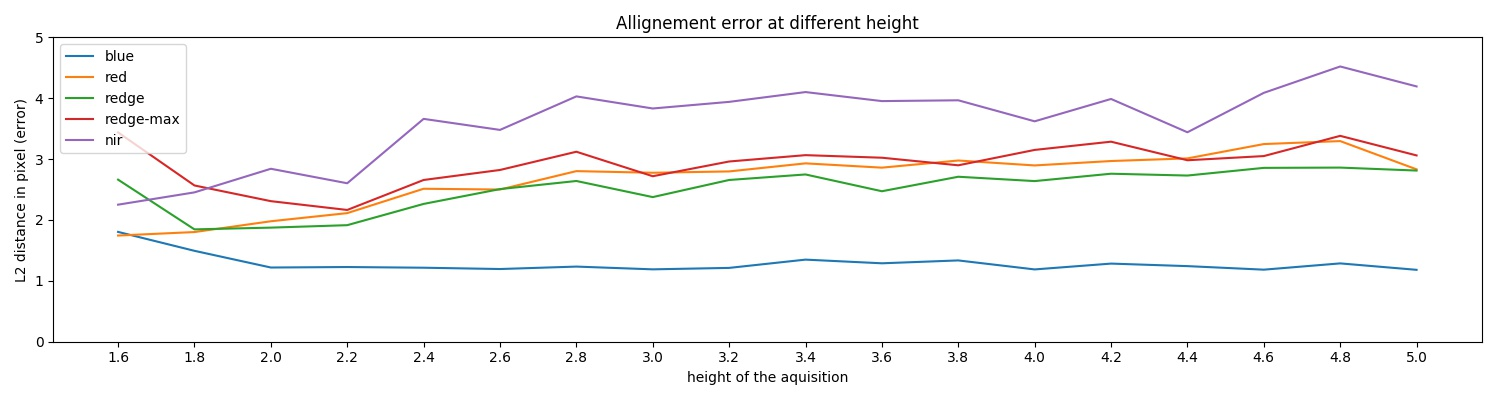
\includegraphics[width=0.8\linewidth]{../figures/affine-allignement-rmse.jpg}
		\caption{The mean distance of detected keypoint before perspective correction}
		\label{fig:affine-error}
	\end{figure}
	
	% https://www.lfd.uci.edu/~gohlke/code/imreg.py.html
	
	\subsection{Perspective correction}
	
	The appendix figure \ref{fig:features-performances} shows the numbers of keypoints after filtering and homography association (minimum of all matches),
	the computation time and performance ratio (matches/time) for each method.
	All these methods work, the choice of method depends on how we want to balance between computation time and accuracy:
	\begin{itemize}
		\item GFTT show the best performance over all others both in computation time and number of matches
		\item FAST and AGAST is suitable too, balanced between time and matches performances.
	\end{itemize}
	
	\noindent
	The other ones did not show improvement in term of performances or matches:
	\begin{itemize}
		\item KAZE show correct number of matches (>200) but it's also 2.5 times slower than FAST and AGAST.
		\item AKAZE and MSER did not show benefits comparing to FAST.
		\item ORB could be excluded, the number of matches is near to 20 how is the minimal to ensure that the homography is correct.
		\item SURF the number of detected feature may not be enough to fit the perspective correction.
		\item BRISK show good number of matches, but there computation time is too huge (79 sec).
	\end{itemize}
	
	\par Increasing the number of key points matched allows a slightly higher accuracy. For example, switch from SURF (30 results) to FAST (130 results). show the final residual distances reduced from ~1.2px to ~0.9px but the calculation time from ~5sec to ~8sec.
	\\
	\par All methods show that the best reference spectrum is 710nm, with the exception of SURF and GFTT which is 570nm.
	The appendix figure \ref{fig:features-FAST-performances} shows the minimum number of matches between each reference spectrum and all others using the FAST algorithm.
	Choosing the right spectral reference is important, as we can see, no correspondence is found in some cases between 650nm-850nm,
	but correspondences are found between 675nm-710nm and 710nm-850nm, making the 710nm more appropriate,
	the same behaviour can be observed for the other bands and 570nm.
	This is visible on the "all\_min" line, 570nm and 710nm have the best minimum number of matches.
	Other best spectral reference are available in supplementary material.
	\\
	\par Residues of the perspective correction show that we have correctly registered each spectral band with a residual error of less than 1 pixel,
	the figure \ref{fig:perspective-error} shows the residual distance at different ground distances.
	
	\begin{figure}[H]
		\centering
		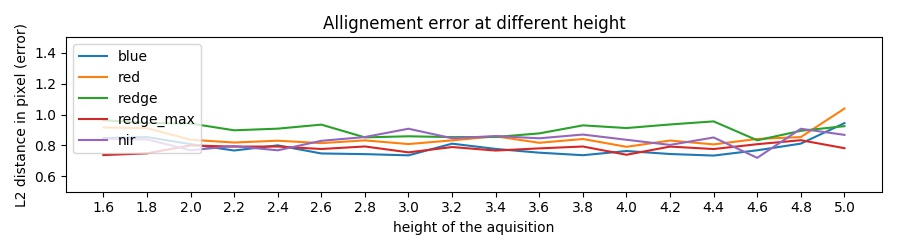
\includegraphics[width=0.8\linewidth]{../figures/prespective-allignement-rmse.jpg}
		\caption{Perspective Re-projection Error}
		\label{fig:perspective-error}
	\end{figure}
	
	\par The appendix figure \ref{fig:perspective-features-matching-scatter} shows the difference between detected points for two bands (red-green)
	before (left) and after (right) the perspective correction, and show that the residual errors are spatially uniform.
	\\
	\par The decomposition of the residual distances by angles $[0-40-80-120-160-200-240-280-320-0]$, visible in the appendix figure \ref{fig:residual-angle} is interesting.
	We can notice that the spatial distribution of the residues, for each different angle, is equally distributed.
	Our hypothesis is that the nature of the base information (spectral band + different lens) makes a small difference to the gradient break,
	which is detected by the features detector and propagated until the final correction (observed residue).
	This is interesting because these residues uniformly distributed by angle in space tend to minimize the resulting correction of its center (gradient),
	thus the detected residual error are overrated and should be less than $0.4$ pixel.

	\subsection{General discussion}
	
	\par Even if the relief of the scene is not taken into account due to the used deformation model,
	in our case we didn't see any difference.
	However, more complex deformation models \cite{Lombaert, ThinPlateSpline} can be used to improve the remaining error.
	This type of complex deformation has not been fully evaluated, but only quickly tested through \textit{cv2.ThinPlateSplineShapeTransformer}.
	There does not seem to be any significant improvement in most cases (with a huge computation time).
	But can also, in some cases, create large angular deformations caused by the proximity of keypoints,
	of course, it's possible to filter these keypoints, which also reduces the overall accuracy.
	\\
	\par Further researches can be performed on each parameter of the feature extractors, for those who need specific performance (time/precision),
	And we invite the one how need it to download the repository and test various combination.
	Otherwise feature matching can be optimized, at this stage, we use brute-force matching with post filtering,
	but a different implementation that fulfill our epipolar line properties should greatly enhance the number of matches by reducing false positives.
	
	
	%%%%%%%%%%%%%%%%%%%
	
	\section{Conclusion}
	
	In this work, the application of different techniques for multi-spectral image registration was explored.
	We tested different methods of keypoints extractors at different heights and the number of control points obtained.
	As seen in the method, the most suitable method is the GFTT with a significant number of matches and a reasonable calculation time.
	\\
	\par Furthermore, the best spectral reference was defined for each method, for example 570 for GFTT.
	According to the figure \ref{fig:perspective-error} we observe a residual error of less than 1 px,
	supposedly caused by the difference in input (spectral range, lens).
	Finally, the method was tested on more than 8000 images in real conditions (not present in the study),
	randomly taken between 1.6 and 2.2 meters without registration error (always a minimum number of matches, without observed error, less than $0.9$px).
	
	\newpage
	\section{Acknowledgment}
	
	The authors acknowledge support from European Union through the project H2020 IWMPRAISE \footnote{\url{https://iwmpraise.eu/}}
	(Integrated Weed Management: PRActical Implementation and Solutions for Europe)
	and from ANR Challenge ROSE through the project IROSEAU \footnote{\url{http://challenge-rose.fr/en/projet/roseau-2/}} (RObotics SEnsorimotor loops to weed AUtonomously).
	
	We would like to thanks Jones Gawain, Combaluzier Quentin, Michon Nicolas, Savi Romain and Jean-Benoit Masson
	for the realization of the metallic gantry that help us for positioning the camera at different heights.
	
	\section{Supplementary material}
	
	The additional data and source code associated with this article can be found in the online version at the following address
	\url{gitlab.com/phd-thesis-adventice/phd-airphen-alignment} the access is limited,
	and we invite you to send an email to the author for full access.
	
	\section{Appendix}

	\begin{figure}[H]
		\centering
		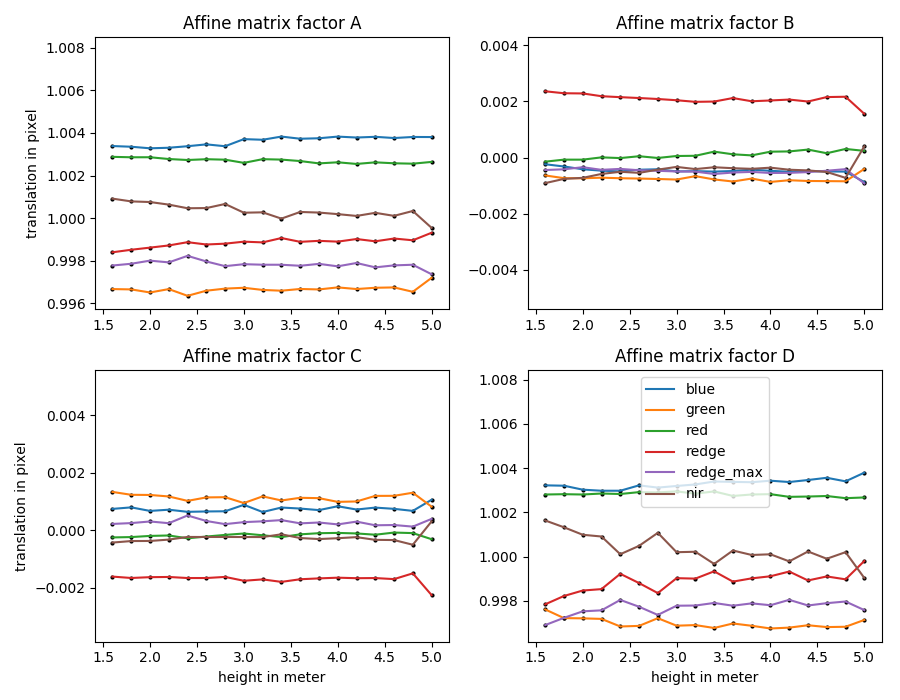
\includegraphics[width=0.6\linewidth]{../figures/affine-rotation-height.png}
		\caption{Affine matrix value by height}
		\label{fig:affine-rotation-height}
	\end{figure}

	\begin{figure}[H]
		\centering
		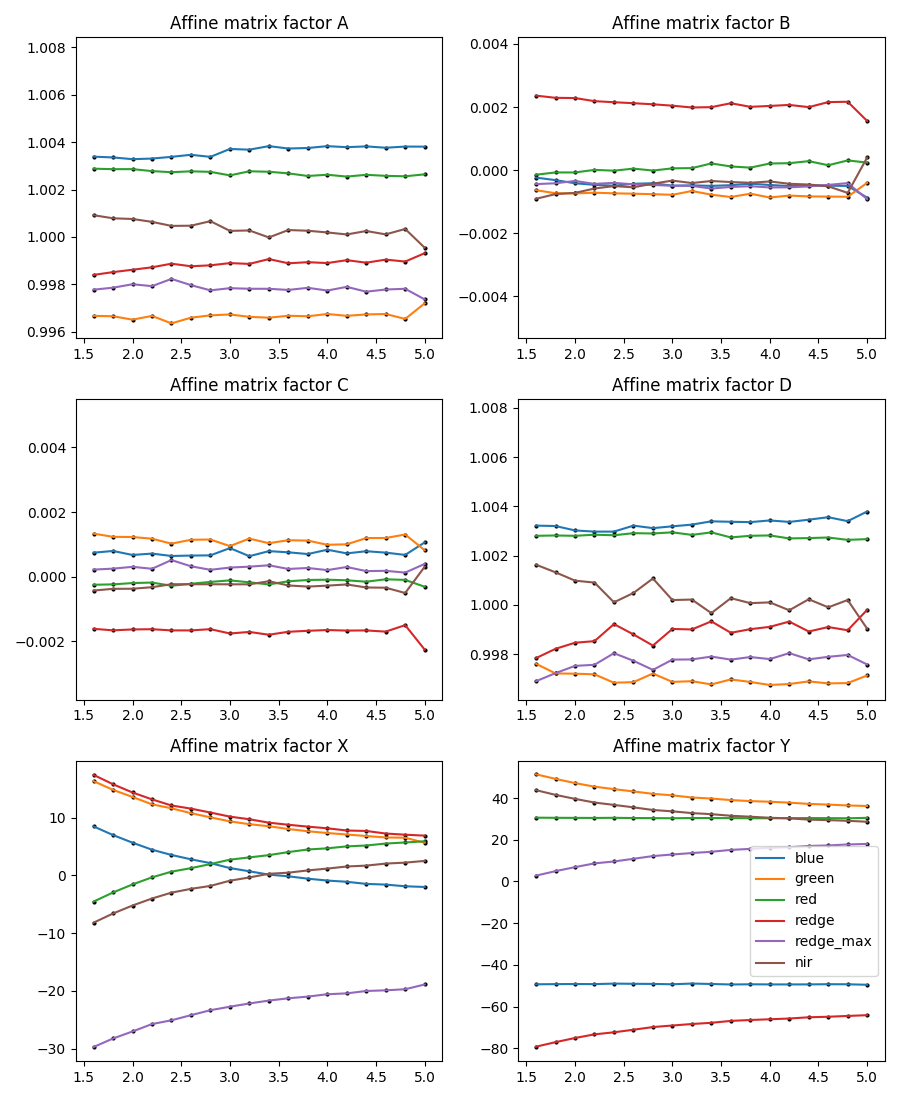
\includegraphics[width=0.6\linewidth]{../figures/affine-translation-height.png}
		\caption{Affine matrix value by height}
		\label{fig:affine-translation-height}
	\end{figure}
	
	\begin{figure}[H]
		\centering
		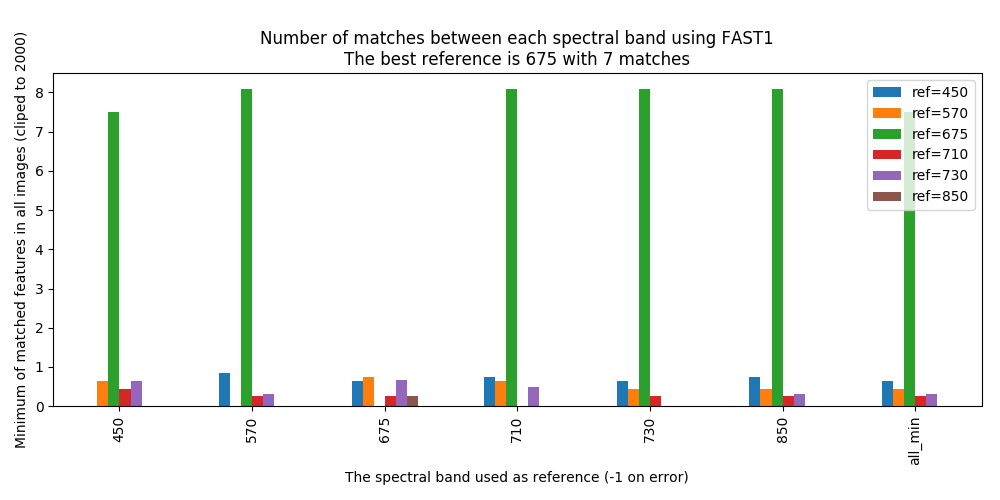
\includegraphics[width=0.7\linewidth]{../figures/comparaison-keypoint-matching-reference-FAST1.png}
		\caption{feature FAST performances}
		\label{fig:features-FAST-performances}
	\end{figure}

	\begin{figure}[H]
		\centering
		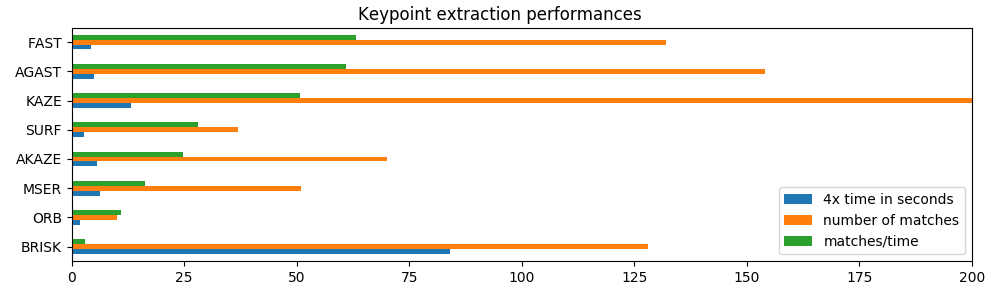
\includegraphics[width=0.7\linewidth]{../figures/comparaison-keypoint-performances.png}
		\caption{features performances}
		\label{fig:features-performances}
	\end{figure}

	\begin{figure}[H]
		\centering
		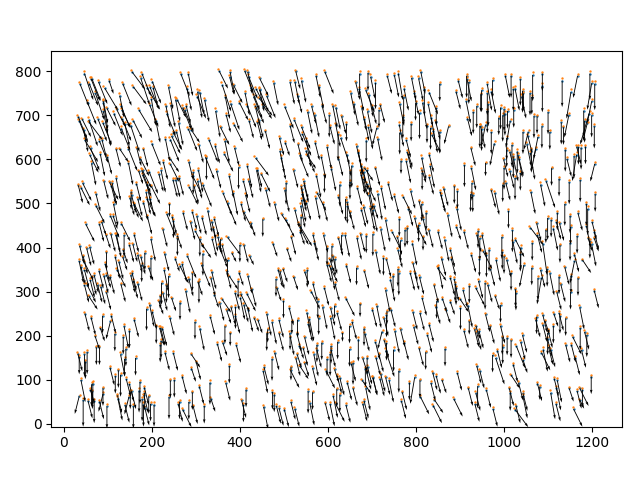
\includegraphics[width=\linewidth]{../figures/perspective-features-matching-scatter.png}
		\caption{perspective-features-matching-scatter}
		\label{fig:perspective-features-matching-scatter}
	\end{figure}

	\begin{figure}[H]
		\centering
		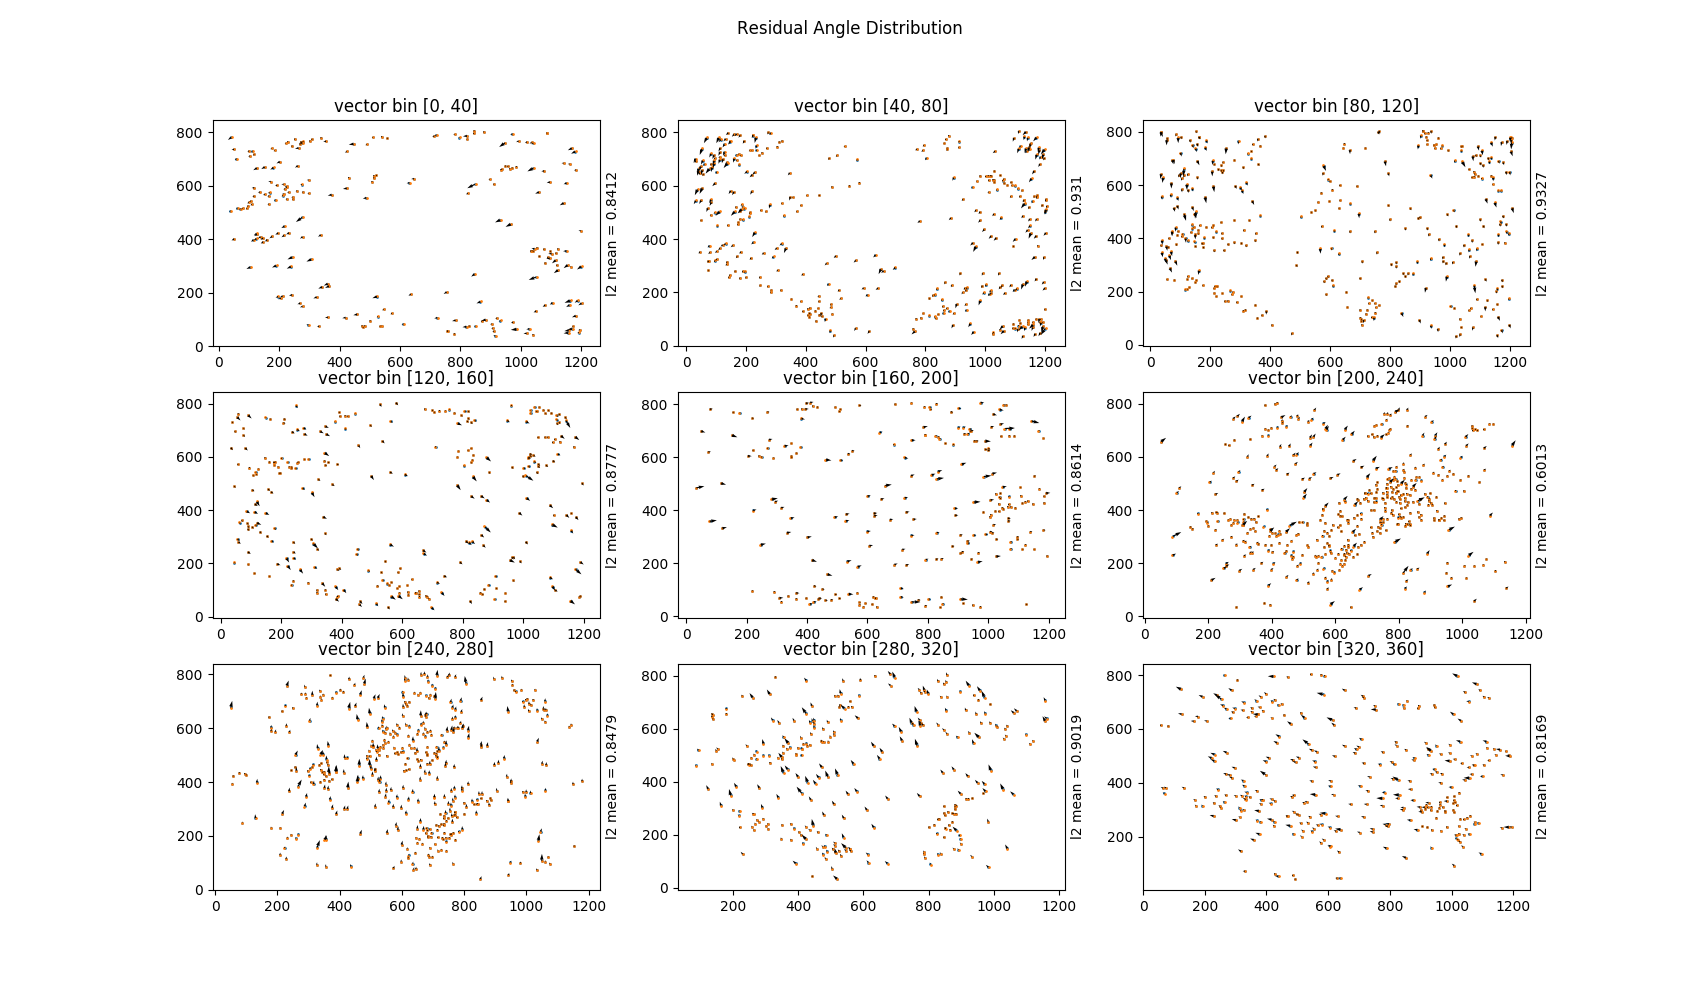
\includegraphics[width=\linewidth]{../figures/perspective-features-residual.png}
		\caption{Residual Distribution Again Angle}
		\label{fig:residual-angle}
	\end{figure}

	\begin{table}[H]
	\begin{tabular}{|l|c|c|c| } 
		\hline
		ABRV & 1 & 2 & 3 \\
		\hline
		ORB & nfeatures=5000 & nfeatures=10000 & nfeatures=15000 \\
		GFTT & maxCorners=5000 & maxCorners=10000 & maxCorners=15000 \\
		AGAST & threshold=71 & threshold=92 & threshold=163 \\
		FAST & threshold=71 & threshold=92 & threshold=163 \\
		AKAZE & nOctaves=1, nOctaveLayers=1 & nOctaves=2, nOctaveLayers=1 & nOctaves=2, nOctaveLayers=2 \\
		KAZE & nOctaves=4, nOctaveLayers=2 & nOctaves=4, nOctaveLayers=4 & nOctaves=2, nOctaveLayers=4 \\
		BRISK & nOctaves=0, patternScale=.1 & nOctaves=1, patternScale=.1 & nOctaves=2, patternScale=.1  \\
		SURF & nOctaves=1, nOctaveLayers=1 & nOctaves=2, nOctaveLayers=1 & nOctaves=2, nOctaveLayers=2 \\
		MSER & & & \\
		\hline
	\end{tabular}
	\caption{list of algorithms with 3 variation of their parameters}
	\label{tab:used-algorithms}
	\end{table}
	
	\section{Reference}
	\bibliography{references.bib}
	\bibliographystyle{apalike}
	
\end{document}
